\documentclass[a4paper]{article}

  \usepackage{fullpage} % Package to use full page
  \usepackage{parskip} % Package to tweak paragraph skipping
  \usepackage{tikz} % Package for drawing
  \usepackage{amsmath}
  \usepackage{siunitx}
  \usepackage{amsfonts}
  \usepackage{amssymb}
  \usepackage{hyperref}
  \usepackage[utf8]{inputenc}
  \usepackage[english]{babel}
  \usepackage{multicol}
  \usepackage{graphicx}
  \graphicspath{ {./images/} }
  
  \newcommand\tab[1][0.5cm]{\hspace*{#1}}
  
  \title{Laboratory 1}
  \author{Adrian Darian, Elaine Huang, Federico Del Castillo Carnero}
  \date{9/2/2020}
  
  \begin{document}
  
\maketitle
  
\section*{Objectives}
\begin{itemize}
	\item Learn how to use Simscape within Matlab and Simulink environment to model and simulate circuits.
	\item Observe the responses of the circuits when the circuits and parameters are changed.
\end{itemize}

\section*{Equipment and Components}
\begin{itemize}
	\item A deak computer
	\item Matlab software
\end{itemize}

\section*{Preliminary}
Simscape™ provides an environment for modeling and simulating physical systems in mechanical, electrical, hydraulic, and other physical domains. It is a set of block libraries and special simulation features for modeling these physical systems.  You can parameterize your models using MATLAB variables and expressions, and design control systems for your physical systems in Simulink. 
  
Simscape provides fundamental building blocks from these domains that you can assemble into models of physical components.  These blocks represent basic mathematical operations. When you connect these blocks together, the resulting diagram is equivalent to the mathematical model, or representation, of the system under design. These connection ports are nondirectional. They mimic physical connections between elements.
  
For circuit simulations, Simscape provides building blocks for circuit elements, such as DC/AC voltage sources, DC/AC current sources, resistors, inductors, capacitors, and switches.
  
Read the “User’s Guide of Simscape” file attached with the lab if necessary.
  
Fill up the table below based on the given circuit and the value of the voltage source.

\section*{Procedure}
\begin{itemize}
	\item[1] Go to \href{https://it.ucmerced.edu/software-list/}{https://it.ucmerced.edu/software-list/} to download Matlab.
	\item[2] Open Matlab from the All Program.
	\item[3] Type simulink in the Matlab Command Window and Simulink Library Browser will be popped up.
	\item[4] Expand the Simscape entry in the contents tree. The Simscape has two top-level libraries: Foundation and Utilities.
	\item[5] Click Foundation library, you will see the libraries for different systems.
	\item[6] Click Electrical, you will see three sub-libraries: Electrical Elements, Electrical Sensors, and Electrical Sources.
	\item[7] Use the blocks provided in these three sub-libraries and the Utilities to build the following circuit.
	      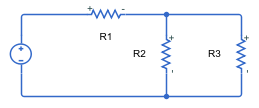
\includegraphics{circuit.png}
	\item[8] Add Current Sensor and Voltage Sensor into your model.
	\item[9] Select your Display from the Sink under the Simulink entry. An example of the circuit model is shown below. \\
	      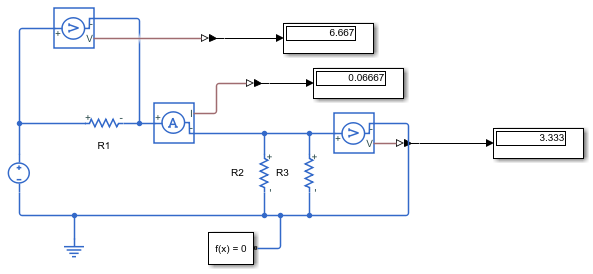
\includegraphics{circuit-final.png}
	\item[10] Set R2 = R3 = \SI{100}{\ohm}. Click the "Resistor 2" in your model. Fill the value of 100 and unit "ohm" in the "Resistance" window. Do the same thing for "Resistor 3".
	\item[11] Set the voltage source to \SI{10}{\volt}.
	\item[12] Change the resistance value of the "Resistor 1" by clicking it in the model. Fill up the following table.      
\end{itemize}

\section*{Analysis of Experimental Data}
\begin{tabular}{|c|c|c|c|}
	\hline
	R1 (\si{\ohm}) & Voltage across R1 (\si{\volt}) & Voltage across R2 (\si{\volt}) & Current flowing through R1 (\si{\ampere}) \\
	\hline
	10             & 1.667                          & 8.333                          & 0.1667                                    \\
	\hline
	20             & 2.857                          & 7.143                          & 0.1429                                    \\
	\hline
	30             & 3.75                           & 6.25                           & 0.125                                     \\
	\hline
	40             & 4.444                          & 5.556                          & 0.1111                                    \\
	\hline
	50             & 5                              & 5                              & 0.1                                       \\
	\hline
	60             & 5.455                          & 4.545                          & 0.09091                                   \\
	\hline
	70             & 5.833                          & 4.167                          & 0.08333                                   \\
	\hline
	80             & 6.154                          & 3.846                          & 0.07692                                   \\
	\hline
	90             & 6.429                          & 3.571                          & 0.07143                                   \\
	\hline
	100            & 6.667                          & 3.333                          & 0.06667                                   \\
	\hline
\end{tabular}

\tab What do you find? Explain them.

\tab\tab Voltage and Current flow throughout the whole circuit diagram. When R1 was less than or equal to \SI{60}{\ohm} the voltage across R2 was greater than the voltage across R1 and then flipped when R1 was greater than \SI{60}{\ohm}. While the current flow just decreases.

\section*{Questions and Conclusions}
\begin{itemize}
	\item Summarize your findings and explanations in this lab. \\
	      During the lab we were instructed to recreate the circuit diagrams shown above in the procedure. Once reconstructed we altered the value of the Resistor 1 so that we may observe the change in voltage across R1 and R2. As well, we got to observe the current flow through R1 in \si{\ampere}. From my calculations, we found that the voltage across R2 was greater than or equal to the voltage across R1 if and only if R1's resistance was \SI{60}{\ohm} or less. Once the resistance of R1 surpassed \SI{60}{\ohm} the voltage across R1 flips and becomes greater than the voltage across R2. As for the current flow across R1, we noticed that as the resistance of R1 increased the flow of current in \si{\ampere} decreased.
\end{itemize}

% ehuang34@ucmerced.edu
% fdelcastillo@ucmerced.edu
  
\end{document}